\documentclass[../main.tex]{subfiles}
\begin{document}

\section{Notation \& Definitions}

%% give the why of the math after every mention of why
 
In this section we introduce a mathematical description of the visualization pipeline where artist $\mathscr{A}$ functions transform data space $\mathscr{E}$ to an intermediate representation in a prerendered graphic space $\mathscr{H}$. 

\begin{equation}
    \label{eq:artist}
    \mathscr{A}: \mathscr{E} \rightarrow \mathscr{H}
\end{equation}

We use fiber bundles\cite{FiberBundle2020, rowlandFiberBundle} to model data and graphics because they allow us to seperate the variables in a dataset from how the values  are connected to each other \cite{butlerVisualizationModelBased1989,butlerVectorBundleClassesForm1992}. The fiber bundles mentioned in this work are assumed to be locally trivial\cite{spanier1989algebraic,LocallyTrivialFibre}. 

We first describe the fiber bundle spaces of data(\ref{sec:data}), graphics(\ref{sec:graphic}), and intermediate visual characteristics (\ref{sec:artist}). We then discuss the equivariant maps between data and visual characteristics (\ref{sec:artist_nu}) and visual characteristics and graphics (\ref{sec:artist_q}) that make up the artist.

\subsection{Data Space}
\label{sec:data}
Lets say we are working with the Global Historical Climatology Network\cite{AnOverviewoftheGlobalHistoricalClimatologyNetworkDailyDatabase}, which is a global daily record of weather station  such as rainfall and temperature. Depending on which aspects of the data we want to visualize, we can encode it as a timeseries or map or both or even represent the measurements as completely disconnected. 

Using a fiber bundle allows us to encode the properties of the heterogenous variables (\ref{sec:data_fiber}), the connectivity of the measurements (\ref{sec:data_base}), and functions between these spaces that yield the measurements (\ref{sec:data_section}).

\subsubsection{Variable Field in F }
\label{sec:data_fiber}
 %%%first sentence should be a paragraph
%%% butler's paper, no notion of distance on K, can only map F to the visual fibers, so need an X to map to Xpos
% variable, measurement, pull in tidy here, 
% % motivate by example, temperature \ time 
%% F_0 = {temp_0, temp_n}, 
%% then adding in a second set of variables time: 
%% F_1 = {time_0, time_1}
% break out into F first as set of values, then F=F_{0}\times F_{1} as component 



The fiber is the cartesian product of the variable spaces:
\begin{align}
F &= F_{0} \times \ldots \times F_{n}
\end{align}

We formulate the fiber such that it has a mapping between the somethine thing and the field name, as discussed in Spivak's simplacial description of databases \cite{spivakSIMPLICIALDATABASES,spivakDatabasesAreCategories2010}. 

Fibers do not need to be 1D.

\subsubsection{Measurement Type}
%% maybe move somewhere else w/ some more motivation
%% do this section in terms of $M0, F_0$
An important property of data fields are the measurement type, which we generalize to identifying the left monoid action such that the monoid actions $M$ 
\begin{equation}
M = M_{0} \times \ldots\times M_{i}
\end{equation}
is the cartesion cross product of monoids applied to each $F_{i}\in F$. A monoid \cite{Monoid2021} $M$ is a set with an associative binary operator $\ast:M \times M\rightarrow M$. A monoid has an identity element $e\in M$ such that $e\ast a= a \ast e = a$ for all $a \in M$. A left monoid action \cite{SemigroupAction2021,ActionNLab} of $M$ is a set $F$ with an action $\bullet: M\times F \rightarrow F$ with the properties:
\begin{description}
    \item[associativity] $\text{for all } m,t \in M \text{ and } x\in F, m\bullet(t\bullet x) = (m\bullet t) \bullet x$
    \item[identity] $\text{for all } x\in F, e\in M,  e\bullet x = x$ 
\end{description} 

The Steven's measurement scales are identified via the group actions on $F_{i}$  \cite{stevensTheoryScalesMeasurement1946, leaFormalizationMeasurementScale} they support. For example, nominal variables are permutable and interval values are translatable. We identify monoid actions, rather than group, to support an extended variety of scales such as partial order. 

%%close out the fiber bundle section with the cartesian products, which gives us heterogenous data , univariate to multivariate. We can decompose the fiber bundle to components bundles \pi:E_1\rightarrow K, .... \pi: E_n\rightarrow K
\subsubsection{Connectivity: Base Space} 
\label{sec:data_base}
%% flows out of the fiber section into, now gluing observations together into a thing
%% can then put functions on edges/planes/etc so we have true continouity
We model data as a fiber bundle ($E$, $K$, $\pi$, $F$)
\begin{equation}
    \label{eq:fiber_bundle}
    \begin{tikzcd}
        F \arrow[r, hook] & E \arrow[r, "\pi"] & K
    \end{tikzcd}
\end{equation}

with topological total space $E$, base space $K$, fiber space $F$, and the map from total space to base space $\pi: E \rightarrow K$. Maps from $K$ to $E$ are called sections and select specific points in $K$. The global space of sections in $E$ is $\Gamma(E)$.

\begin{figure}[h!]
    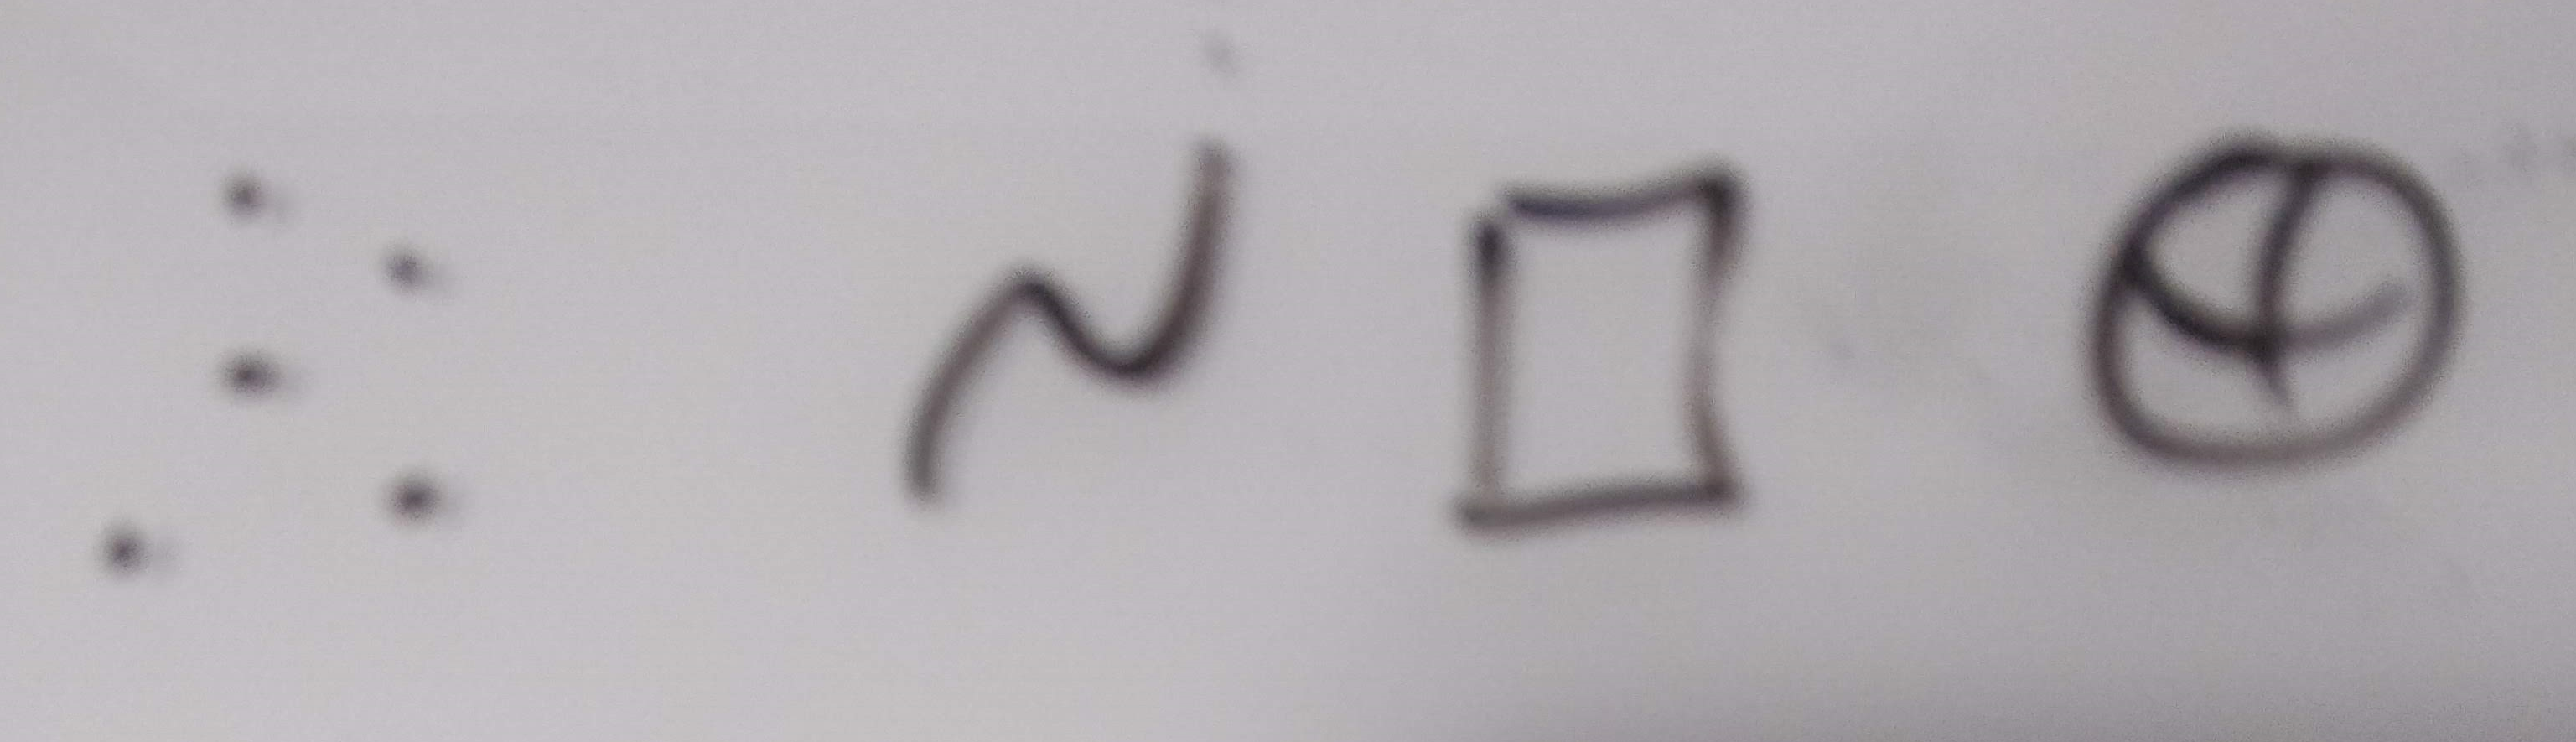
\includegraphics[width=\textwidth]{figures/math/k_different_types.png}
    \label{fig:base_space_types}
    \caption{The topological base space $K$ encodes the connectivity of the data space, for example if the data is independent points or a map or on a sphere}
\end{figure}

Datasets have a semantic topology such as the values are interpreted as discrete observations or part of a timeseries or map, or nodes in a networks \cite{munznerWhatDataAbstraction2014,geveci2012vtk}. %%turn it into a paragraph

As illustrated in fig~\ref{fig:base_space_div}, $K$ is this underlying structure. $K$ does not directly know the values; instead it is the sections that define the lookup between keys $k \in K$ and the corresponding values in $E$.

\begin{figure}[h!]
    \label{fig:base_space_div}
    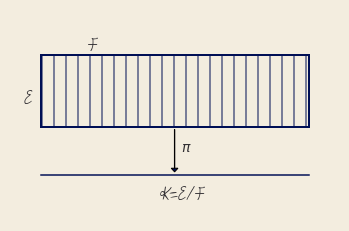
\includegraphics[width=.5\linewidth]{figures/math/k_qspace.png}
    %%include second figure where fiber goes otherway
\end{figure}
The topology $K$ and the

%%this paragraph isn't working
$F$ are determined by how $E$ is subdivided\cite{QuotientSpaceTopology2020,QuotientSpaceTopology2020}. In figure~\ref{fig:base_space_div} we can divide a rectangular base space such that there is a short fiber and long base space or a long fiber and short base space. This is analogous to long and wide forms of the same table \cite{wickham2014tidy}.

\subsubsection{Data: Section}
\label{sec:data_section}
%%% visual variable encoding in a consistent/atomic way in a complex structure 
\label{sec:section_data}
The sections of the fiber bundles are the instances of the data. They are the functions that map from a point $k \in K$ to a set of values in $F$. For example, if we have a database, the section is the table that yields a row given an index. The section $\tau$ is the mapping from base space to total space $\tau: K\rightarrow E$ 
\begin{equation}
    \label{eq:section}
    \begin{tikzcd}
        F \arrow[r, hook] & E \arrow[d, "\pi"']           \\
        & K \arrow[u, "\tau"', bend right]
    \end{tikzcd}
\end{equation}

%%% change to b\c locally trivial, can represent 
such that in a trivial fiber bundle, $E = K \times F$ \cite{rowlandFiberBundle,FiberBundle2020}:
\begin{equation}
    \label{eq:section_return}
    \tau(k) = (k, (x_{F_{0}}, \ldots, x_{F_{n}}))
\end{equation}

%%%can decompose bundles into Ei such that \tau: E_{i} \rightarrow K, where F_{i} is the fiber of E_{i}
which we can also decompose such that
\begin{align}
\tau_{0}(k) &= (k, (x_{F_{0}}))\\
            & \vdotswithin{=}\\
\tau_{n}(k) &= (k, (x_{F_{n}}))
\end{align}

which allows us to have field wise access to the data so long as there is a shared $K$.  
%% we will use this property later for visual mapping such that we can seperate each variable into its own bundle

\subsubsection{Sheaf and Stalk}
\label{sec:data_sheaf_stalk}
%%% sheaf is how we break up the base space 
Often a graphic may need to be updated with live data or support zooming in on a segement of the dataset; to support working with a subset of data, we can use the sheaf $\mathcal{O}(E)$

\begin{equation}
    \label{eq:sheaf}
    \begin{tikzcd}
        \iota^*E \arrow[d, "\pi"']           & E \arrow[d, "\pi"'] \arrow[l, "\iota^*"']         \\
        U \arrow[u, "\iota^*\tau"', bend right] & K \arrow[u, "\tau"', bend right] \arrow[l, "\iota"']
        \end{tikzcd}
\end{equation}
which is the localized section of fibers $\iota^*\tau: U \rightarrow \iota^*E$ pulled back via the inclusion map $\iota: U \rightarrow K$. The localized section is the germ $\xi^*\tau$. The neighborhood of points $k_i$ surrounding the point $k$ the sheaf lies over is the stalk $\mathcal{F}_b$ \cite{StalkSheaf2019,spanier1989algebraic}.

%% the stalk contains all the local information, typically we only need some of the information, such as the firtst or second direivative. in practice we only need the jet which is...in practive will extend the fiber 
The jet bundle $\mathcal{J}$ \cite{JetBundle2020,musilovaCalculusVariationsJet2016} is a for writing differential equations on sections of fiber bundles; this information is required for some visual characteristics, such as line thickness. 

\subsubsection{Example: Temperature}
\textcolor{red}{Moved \& walked through b/c was getting clunky to not have terms yet}\\

% can't make a 1D fiber - can't make a 1D fiber, switch the picture to plane over 0D and 1D and then can talk about disconnected or connected

% break out the mbox/clean up the typesetting
The fiber bundle model is flexible enough to express some of the many different forms that temperature data can come in. 

\begin{figure}[h!]
    \begin{subfigure}{.5\textwidth}
        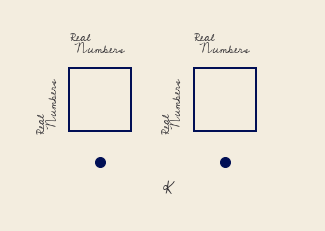
\includegraphics[width=\textwidth]{figures/math/temp_1k.png}
        %% add box around neighboring P and Map
        \label{fig:base_example_line}
    \end{subfigure}
    \begin{subfigure}{.5\textwidth}
        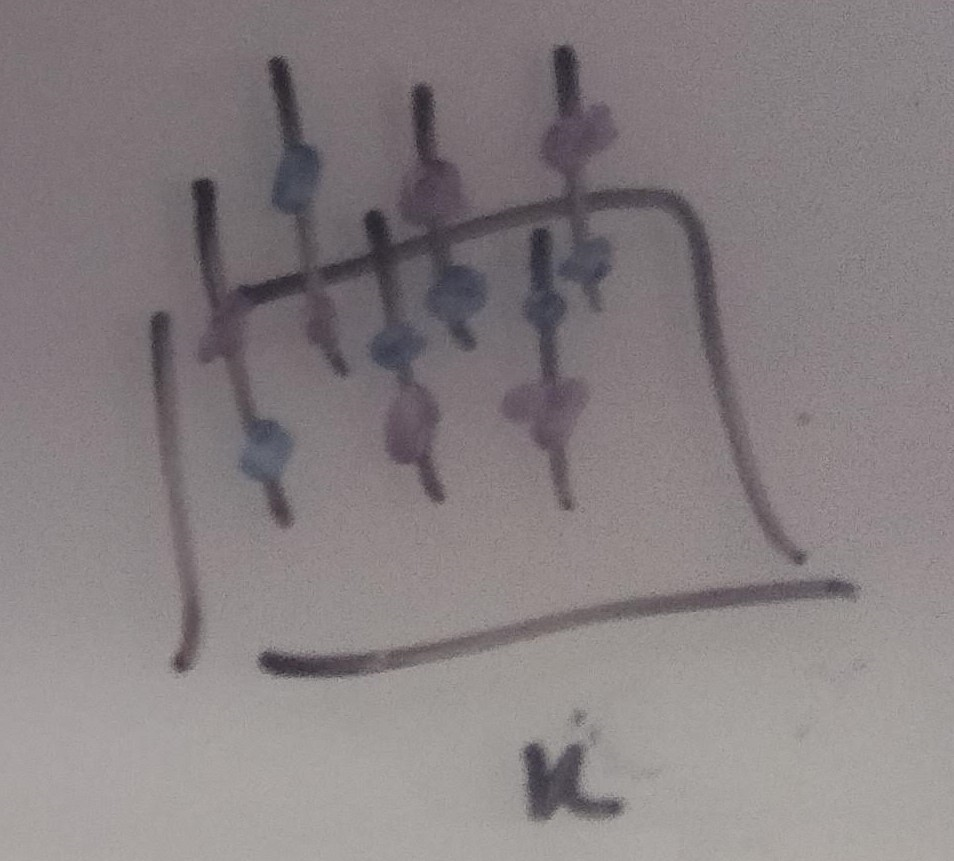
\includegraphics[width=\textwidth]{figures/math/temp_2k.png}
        \label{fig:base_example_plane}
    \end{subfigure}
    \label{fig:base_example}
    \caption{These two datasets have the same fiber of temperature but different base spaces. In figure~\ref{fig:base_example_line} the temperature values are 1D continuous, while in figure~\ref{fig:base_example_plane} the temperature values are 2D continuous.}
\end{figure}

The datasets in figure~\ref{fig:base_example} have identical fibers that encode a set of temperature values. In figure~\ref{fig:base_example_line} the temperatures lie on a line such that a section could return a timeseries or a distribution. In figure~\ref{fig:base_example_plane}, the temperatures lie on a 2D continuous plane; a section could return a map or contour. Because the fiber is 1D, it does not encode metadata 

\begin{figure}[h!]
    \begin{subfigure}{.5\textwidth}
        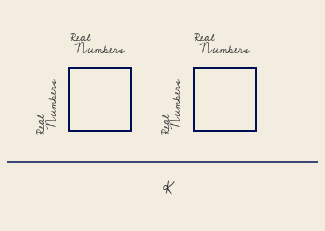
\includegraphics[width=\textwidth]{figures/math/temp_2f.png}
        \label{fig:fiber_example_plane}
    \end{subfigure}
    \begin{subfigure}{.5\textwidth}
        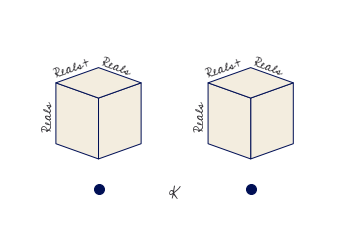
\includegraphics[width=\textwidth]{figures/math/temp_3f.png}
        \label{fig:fiber_example_cube}
    \end{subfigure}
    \label{fig:fiber_example}
    \caption{The fiber is expanded to include metadata fields that describe the semantics of $K$. In figure~\ref{fig:fiber_example_plane} the fiber is \textrm{temperature} $\times$ \textrm{time} and in figure~\ref{fig:fiber_example_cube} the fiber is \textrm{temperature}$\times$ \textrm{latitude} $\times$ {longitude}}.
\end{figure}

To encode the metadata, the fiber is expanded as illustrated in figure~\ref{fig:fiber_example}. The fiber in figure~\ref{fig:fiber_example_plane} is the cartesian product of the space of possible temperature values in degrees celsius and space of possible time values
\begin{equation}
F = [temp_{min}, temp_{max}] \times [time_{min}, time_{max}]
\label{eq:fiber_plane}
\end{equation}

while the fiber in figure~\ref{fig:fiber_example_cube} is the cartesian product of temperature, latitude, and longitude
\begin{equation}
F = [temp_{min}, temp_{max}] \times [-90, 90] \times [-180, 180]
\label{eg:fiber_cube}
\end{equation}

such that $E$ is the space of all possible points in $F$.

\begin{figure}[h!]
    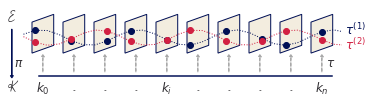
\includegraphics[width=1\linewidth]{figures/math/fiberbundle.png}
    \label{fig:fiber_example_section}
    \caption{The section $\tau_1$ returns the blue points,  while $\tau_2$ returns the purple points. $\Gamma(E)$ is the set of all sections, including $\tau_1$ and $\tau_2$}.  
\end{figure}
Given the fiber described in equation~\ref{eq:fiber_plane}, the sections $\tau_{1}$ and $\tau_{2}$ in figure~\ref{fig:fiber_example_section} return tuples of the form
\begin{equation}
\tau(k) = (k, (temperature, time))
\end{equation}
such that sections with the constraint that time is monotonic return a timeseries. 


\subsection{Prerender Space $H$}
\label{sec:graphic}
We define a graphic space $H$ such that we do not have to assume the physical output space of the renderer. This means that the graphic in $H$ can be output to a screen or 3D printed space or a dome. We model the prerender space as a fiber bundle (H, S, $\pi$, D). $H$ is the predisplay space, with a fiber $D$ dependent on the target display and a base space of $S$. 

\subsubsection{Base space}
The underlying topology $S$ of a graphic often needs more dimensions than the data topology $K$ because of the specifications of the display space. For example, a line plot on a plane (such as a screen or a piece of paper) by necessity needs to also have a thickness so that it is visible, which maps back to a set of connected points in $H$. The topology of these connected points is therefore the region $s \subset S$ such that $\xi: S \rightarrow K$ is a deformation retraction \cite{RetractionTopology2020}
\begin{equation}
    \begin{tikzcd}
        E \arrow[d, "\pi"'] & H \arrow[d, "\pi"'] \\
        K                   & S \arrow[l, "\xi"']
        \end{tikzcd}
\end{equation}

that goes from a region $s \in S_{k}$ to its associated point $k$, such that when $\xi(s) = k$, $\xi^*\tau(s) = \tau(k)$. 

\subsubsection{Fiber and Section}
A section $\rho: S \rightarrow H$ is a mapping from a region $s$ on a mathematical encoding of the image to a region $xy$ on the screen that the renderer then maps to visual space as defined in D.

\paragraph{Example}
For a physical screen display, we can consider a predisplay space that is a trivial fiber bundle $H=\mathbb{R}^{5}\times S$ such that $\rho$ is
\begin{equation}
    \rho(s)  = [x(s), y(s), r(s), g(s), b(s)]
    \label{eq:rho}
\end{equation}

To draw an image, a region, $H$ is inverse mapped into a region $s \in S$ where
\begin{equation}
s = \rho^{-1}_{\tiny{XY}}(xy)
\end{equation}
such that the rest of the fields in $\mathbb{R}^{7}$ are then integrated over $s$ to yield the remaining fields:
\begin{align}
    r &= \iint\limits_s \rho_{\tiny{R}}(s)ds^{2}\\
    g &= \iint\limits_s \rho_{\tiny{G}}(s)ds^{2}\\
    b &= \iint\limits_s \rho_{\tiny{B}}(s)ds^{2}
\end{align}

Here we assume a single opaque 2D image such that the $z$ and $alpha$ fields can be omitted. To support overplotting and transparency, we can consider $D=R^{7}$

\subsubsection{{Example}}
\begin{figure}[h!]
    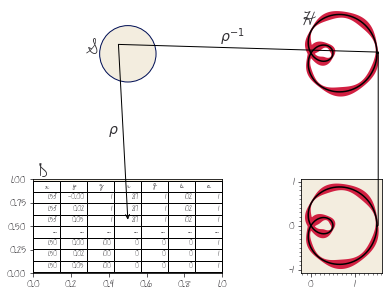
\includegraphics[width=.4\linewidth]{figures/math/render.png}
    \caption{}
    \label{fig:render}
\end{figure}

As illustrated in figure~\ref{fig:render}, words.

\subsection{Artist}
\label{sec:artist}

In this section we will define the artist as a mapping from a sheaf $\mathcal{O}(E)$  to $\mathcal{O}(H)$. 
\begin{equation}
    A: \mathcal{O}(E) \rightarrow \mathcal{O}(H)
\end{equation}

The artist decomposes to mapping data to visual $\nu:E\rightarrow V$, then  compositing $V$ pulled back along $\xi$ to $\xi^*V$ to a visual mark in prerender space $Q:\xi^*V\rightarrow H$. 

\begin{equation}
    \label{eq:artist}
    \begin{tikzcd}
        E \arrow[r, "\nu"] \arrow[rd, "\pi"'] & V \arrow[d, "\pi"] & \xi^*V \arrow[r, "Q"] \arrow[d, "\xi^*\pi"'] \arrow[l, "\xi^*"'] & H \arrow[ld, "\pi"] \\
                                              & K                  & S \arrow[l, "\xi"']                                              &                    
        \end{tikzcd}
\end{equation}
The pullback map $\xi^*$ copies each value in $V$ over $k$ to $s$ in corresponding $S_k$ such that $\xi^*V$ can have multiple values that map to one value in $V$. 

The visual fiber bundle ($V$, $K$, $\pi$, $P$) has section $\mu: V \rightarrow K$ that resolves to a visual variable \cite{bertinIIPropertiesGraphic2011,munznerMarksChannels,} in fiber $P$. The visual transformer $\nu$ is a set of functions each targeting a different $\mu$
\begin{equation}
    \label{eq:nu_expanded}
    \{\nu_{0}, \ldots, \nu_{n}\}: \{\tau_{0}, \ldots, \tau_{n}\} \mapsto \{\mu_{0}, \ldots, \mu_{n}\}
\end{equation}

where $\mu_{i}$ are the visual parameters in the assembly function $Q(\mu_{0}, \ldots, \mu_{n})(s) = \rho(s)$. 


\subsubsection {Example: Matplotlib Visual Fiber}
For example, for Matplotlib \cite{hunterMatplotlib2DGraphics2007}, some of the possible types in $P$ are:
\begin{table}[ht]
    \renewcommand{\arraystretch}{2}
    \begin{tabulary}{\textwidth}{|l|L|l|}\hline
     $\bm{\nu_{i}}$                      & $\bm{\mu_{i}}$                                                            & $\bm{codomain(\nu_{i})}$  \\ \hline                                              
    position                    & x, y, z, theta, r                                                          & $\mathbb{R}$   \\ \hline
    size                        & linewidth, markersize                                            & $\mathbb{R}^{+}$   \\ \hline
    shape                       & markerstyle                                                      & $\{f_{0}, \ldots, f_{n}\}$ \\ \hline
    color                       & color, facecolor, markerfacecolor, edgecolor  & $\mathbb{R}^{4}$ \\ \hline
    \multirow{2}{*}{texture}    & hatch                                                            & $\mathbb{N}^{10}$\\\cline{2-3}
                                & linestyle                                                        & $\{f_{0}, \ldots, f_{n}\} \times (\mathbb{R}, \mathbb{R^+}^{n, n\%2=0})$ \\ \hline              
    \end{tabulary}
    \label{tab:mpl_visual_variable_fiber}
\end{table}

Table~\ref{tab:mpl_visual_variable_fiber} is an example of the visual fiber defined in terms of common parameters to plots in Matplotlib. The range of $\mu_{i}$ determine the monoid actions on $\mu_{i}$. A section of V $\mu$ is a tuple of visual values that specifies the visual characteristics of a glyph. For example, given a fiber of $\{xpos, ypos, color\}$ one section is $\{.5, .5, (255, 20,147)\}$. $Q$ determines how this section is applied to a graphic.  

\subsubsection{Visual Channels}
\label{sec:artist_nu}
$\nu: E \rightarrow V$ is an equivariant map such that there is a homomorphism from left monoid actions on $E_{i}$ to left monoid actions on $V_{i}$ where $i$ identifies a field in the fiber. $E_i$ and $V_{i}$ each contain a set of values as defined in $F$ and $P$ respectively. A validly constructed $\nu$ is one where the  diagram 
\begin{equation}
    \label{eq:nu_categorical}
\begin{tikzcd}
    E_i \arrow[r] \arrow[r, "\nu_i"] \arrow[d, "m_e"'] & V_i \arrow[d, "m_v"] \\
    E_i \arrow[r, "\nu_i"]                           & V_i               
\end{tikzcd}
\end{equation}
commutes such that $\nu_i(m_e(E_i)) = m_v(\nu_i(E_i))$.

\paragraph{Example: Ordering}
To preserve ordering of elements in $E_i$, $\nu$ must be a monotonic function such that given $e_1, e_2 \in E_{i}$
\begin{equation}
\text{ if } e_1 \leq e_2 \text{ then } \nu(e_1) \leq \nu(e_2)
\end{equation}

\paragraph{Example: Translation}
According to Stevens, interval data is a set with general linear group actions \cite{stevensTheoryScalesMeasurement1946,leaFormalizationMeasurementScale}. Position is a visual variable that can support translation 
\begin{equation}
\nu(x + c) = \nu(x) + \nu(c)
\end{equation}


\paragraph{Example: Invalid $\nu$}
Given a transform $t(x) = x+2$, we construct a $\nu$ that always takes data to .5: 
\begin{equation}
    \label{eq:nu_equation_bad}
    \begin{tikzcd}
        E_1 \arrow[r] \arrow[r, "\lambda:e\mapsto.5"] \arrow[d, "2e"'] & V_i \arrow[d, "2v"] \\
        E_1 \arrow[r, "\lambda"]                                        & V_1                 
    \end{tikzcd}
\end{equation}

This $\nu$ is invalid because the graph does not commute for $t$:
\begin{align}
    \nu(t(e)) & \overset{?}{=} t(\nu(e))\\
    .5 & \overset{?}{=} t(.5)\\
    .5 & \neq 2*.5
\end{align}

To construct a valid $\nu$, the diagram must commute for all monoid actions on the sets in $E_i, V_i$.


\subsubsection{Assembling Marks}
\label{sec:artist_q}
\begin{figure}[h!]
    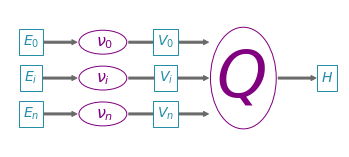
\includegraphics[width=\textwidth]{figures/math/path_of_q}
    \label{fig:artist_q}
    \caption{The $\nu$ functions convert data $E$ to visual $V$. $Q$ assembles the different types of visual parameters $V_{i}$ into a graphic in $H$. $Q\circ\mu(\xi^{-1}J)$ forms a visual mark by applying $Q$ to a region mapped to connected components $J \subset K$.}  
\end{figure}

As shown in figure~\ref{fig:artist_q}, $Q$ takes the individual fields in $V$ as input and outputs a single piece of a graphic on $H$. As with $\nu$, the constraint on $Q$ is that for every monoid actions on the input in $V$ there is a corresponding monoid action on the output in $H$
\begin{equation}
    Q: \Gamma(V) \rightarrow \Gamma(H)
\end{equation}
When $Q: \mu \mapsto \rho$ yields a $\rho$ that maps to the same values in $D$ over all $S_k$, then $M$ can be defined over $\Gamma(H)$ such that a constraint on $Q$ is that it must be equivariant. For example, when $\mu_{i}$ is the color of the glyph, it maps directly to (R,G,B) in D.

\begin{figure}[h!]
    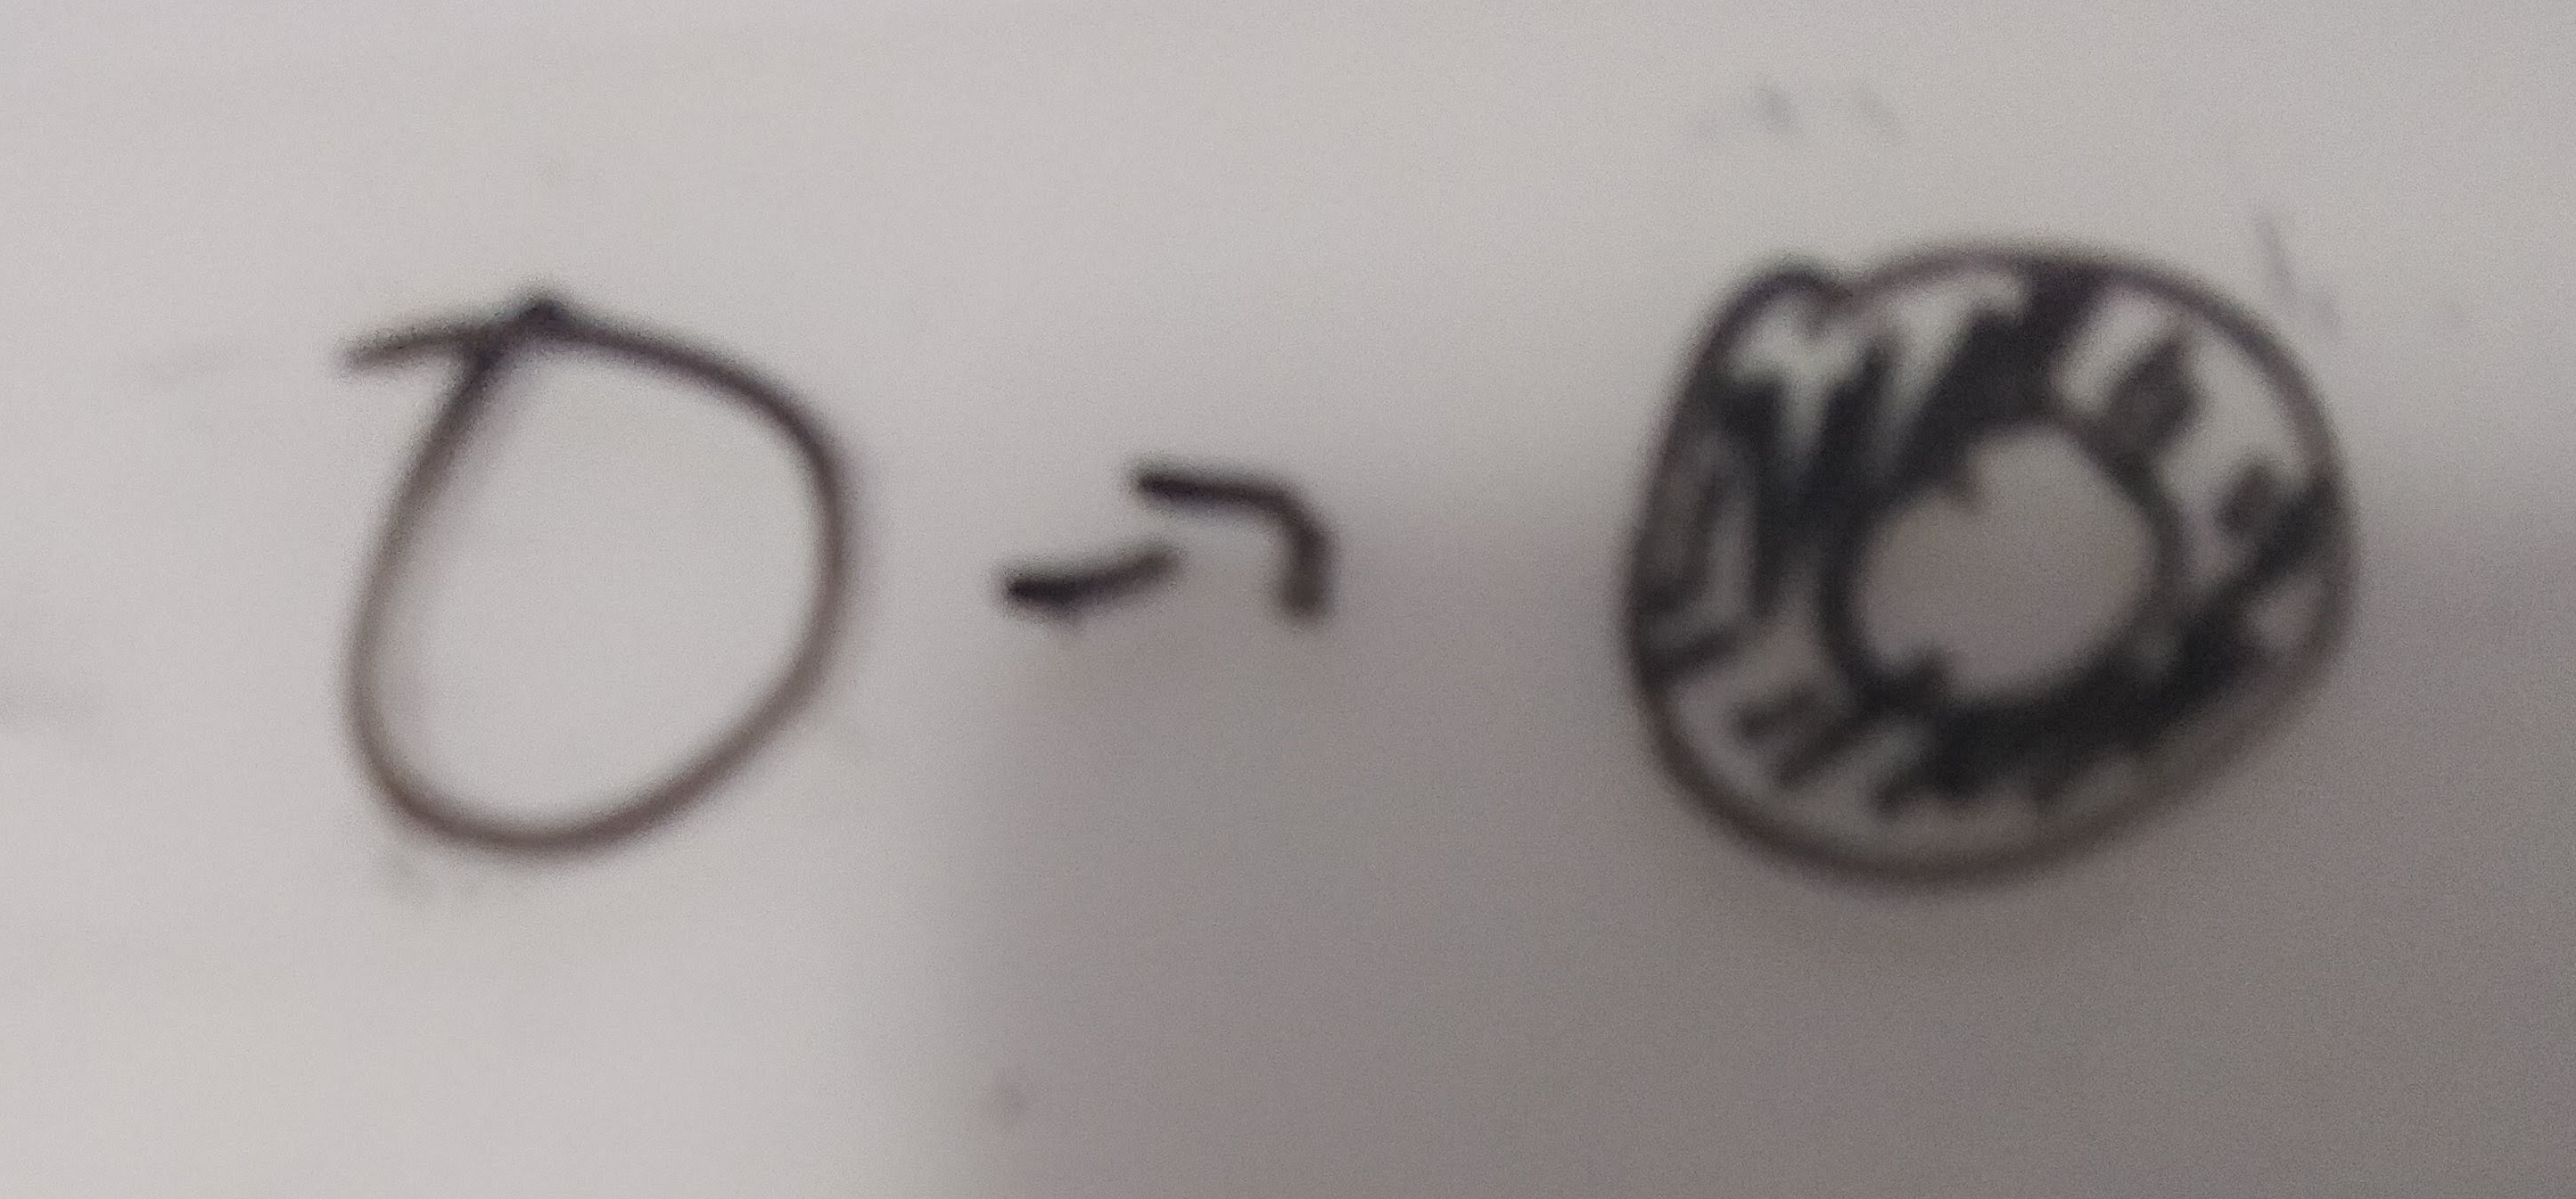
\includegraphics[width=\textwidth]{figures/math/diff_type_q.png}
    \label{fig:artist_mark_change}
\end{figure}

Many $\mu_{i}$ are graphical parameters that do not apply to the whole glyph, such as edge thickness in figure~\ref{fig:artist_mark_change}. 

%%% rework this sentence
In these situations, not all  $\rho$ in $\Gamma(H)$ will support these parameters; instead we define an action on the output graphic $Q(\Gamma(V)) \in \Gamma(H)$ since by definition every section $\mu$ will have a corresponding $\rho$.

We then define the constraint on $Q$ such that if $Q$ applied to two sections $\mu, \mu\prime$ generate the same graphic $\rho$, then the output of both sections acted on by the same monoid $m$ must also be the same.    

Lets call the visual encodings $\Gamma(V)=X$ and the graphic $Q(\Gamma(V))=Y$. If $\forall m \in M$ and $\forall \mu, \mu^\prime \in X$, 
\begin{equation}
Q(\mu) = Q(\mu^\prime)\implies Q(m\circ\mu) = Q(m\circ\mu^\prime)
\end{equation}
then a group action on $Y$ can be defined as $m\circ \rho = \rho^\prime$ where $\rho^\prime=Q(g\circ \mu)$ with $\mu \in Q^{-1}(\rho)$. 

Given  
\begin{itemize}
    \item $P = \{xpos, ypos, color, thickness\}$
    \item $\mu = {0,0,0, 1}$
    \item  $Q(\mu)=\rho$ generates a piece of the thin circle in figure~\ref{fig:artist_mark_change}
\end{itemize}

the constraint on $Q$ means that the translation $m=\{e, e, e, x+2\}$ applied to $\mu$ such that $\mu^\prime=\{0,0,0,3\}$ has an equivalent action on $\rho$ that causes $Q(\mu\prime)$ to be equivalent to the thicker circle in figure~\ref{fig:artist_mark_change}.


\paragraph{Example: Invalid Q}
\textcolor{blue}{Insert some degenerate Q that generates an inconsistent glyph}


Check a well defined map $M\times Y \rightarrow Y$.


constraint: inputs go to same o
utput means changes to inputs mean same changes to output

\paragraph{Graphical Marks}
To output a mark  \cite{bertinIIPropertiesGraphic2011,carpendaleVisualRepresentationSemiology}, $Q$ is called with all the regions $s$ that map back to a set of connected components $J \subset K$:
\begin{equation}
J = \{j \in K \text{ s. t. } \exists \gamma \text{ s.t. } \gamma(0)=k \text{ and }\gamma(1)=j\}
\end{equation}
where the path\cite{ConnectedSpace2020}  $\gamma$ from $k$ to $j$ is a continous function from the interval [0,1].

We define the mark as the graphic generated by $Q(S_j)$

\begin{equation}
    \begin{tikzcd}
        H \arrow[r, shift left] & S_j \arrow[rr, "\xi(s)", shift left] \arrow[l, "\rho(S_j)"] &  & J_{k} \arrow[ll, "\xi^{-1}(J)"]
        \end{tikzcd}
    \label{eq:mark}
\end{equation}

in terms of $K$ because mark is a semantic term denoting the graphic representation of the data.

\subsubsection{Sample Qs}
In this section we formulate the minimal Q that will generate distinguishable graphical marks: non-overlapping scatter points, a non-infinitely thin line, and a simple heatmap. 

\paragraph{Q: scatter plot}
\begin{figure}[h!]
    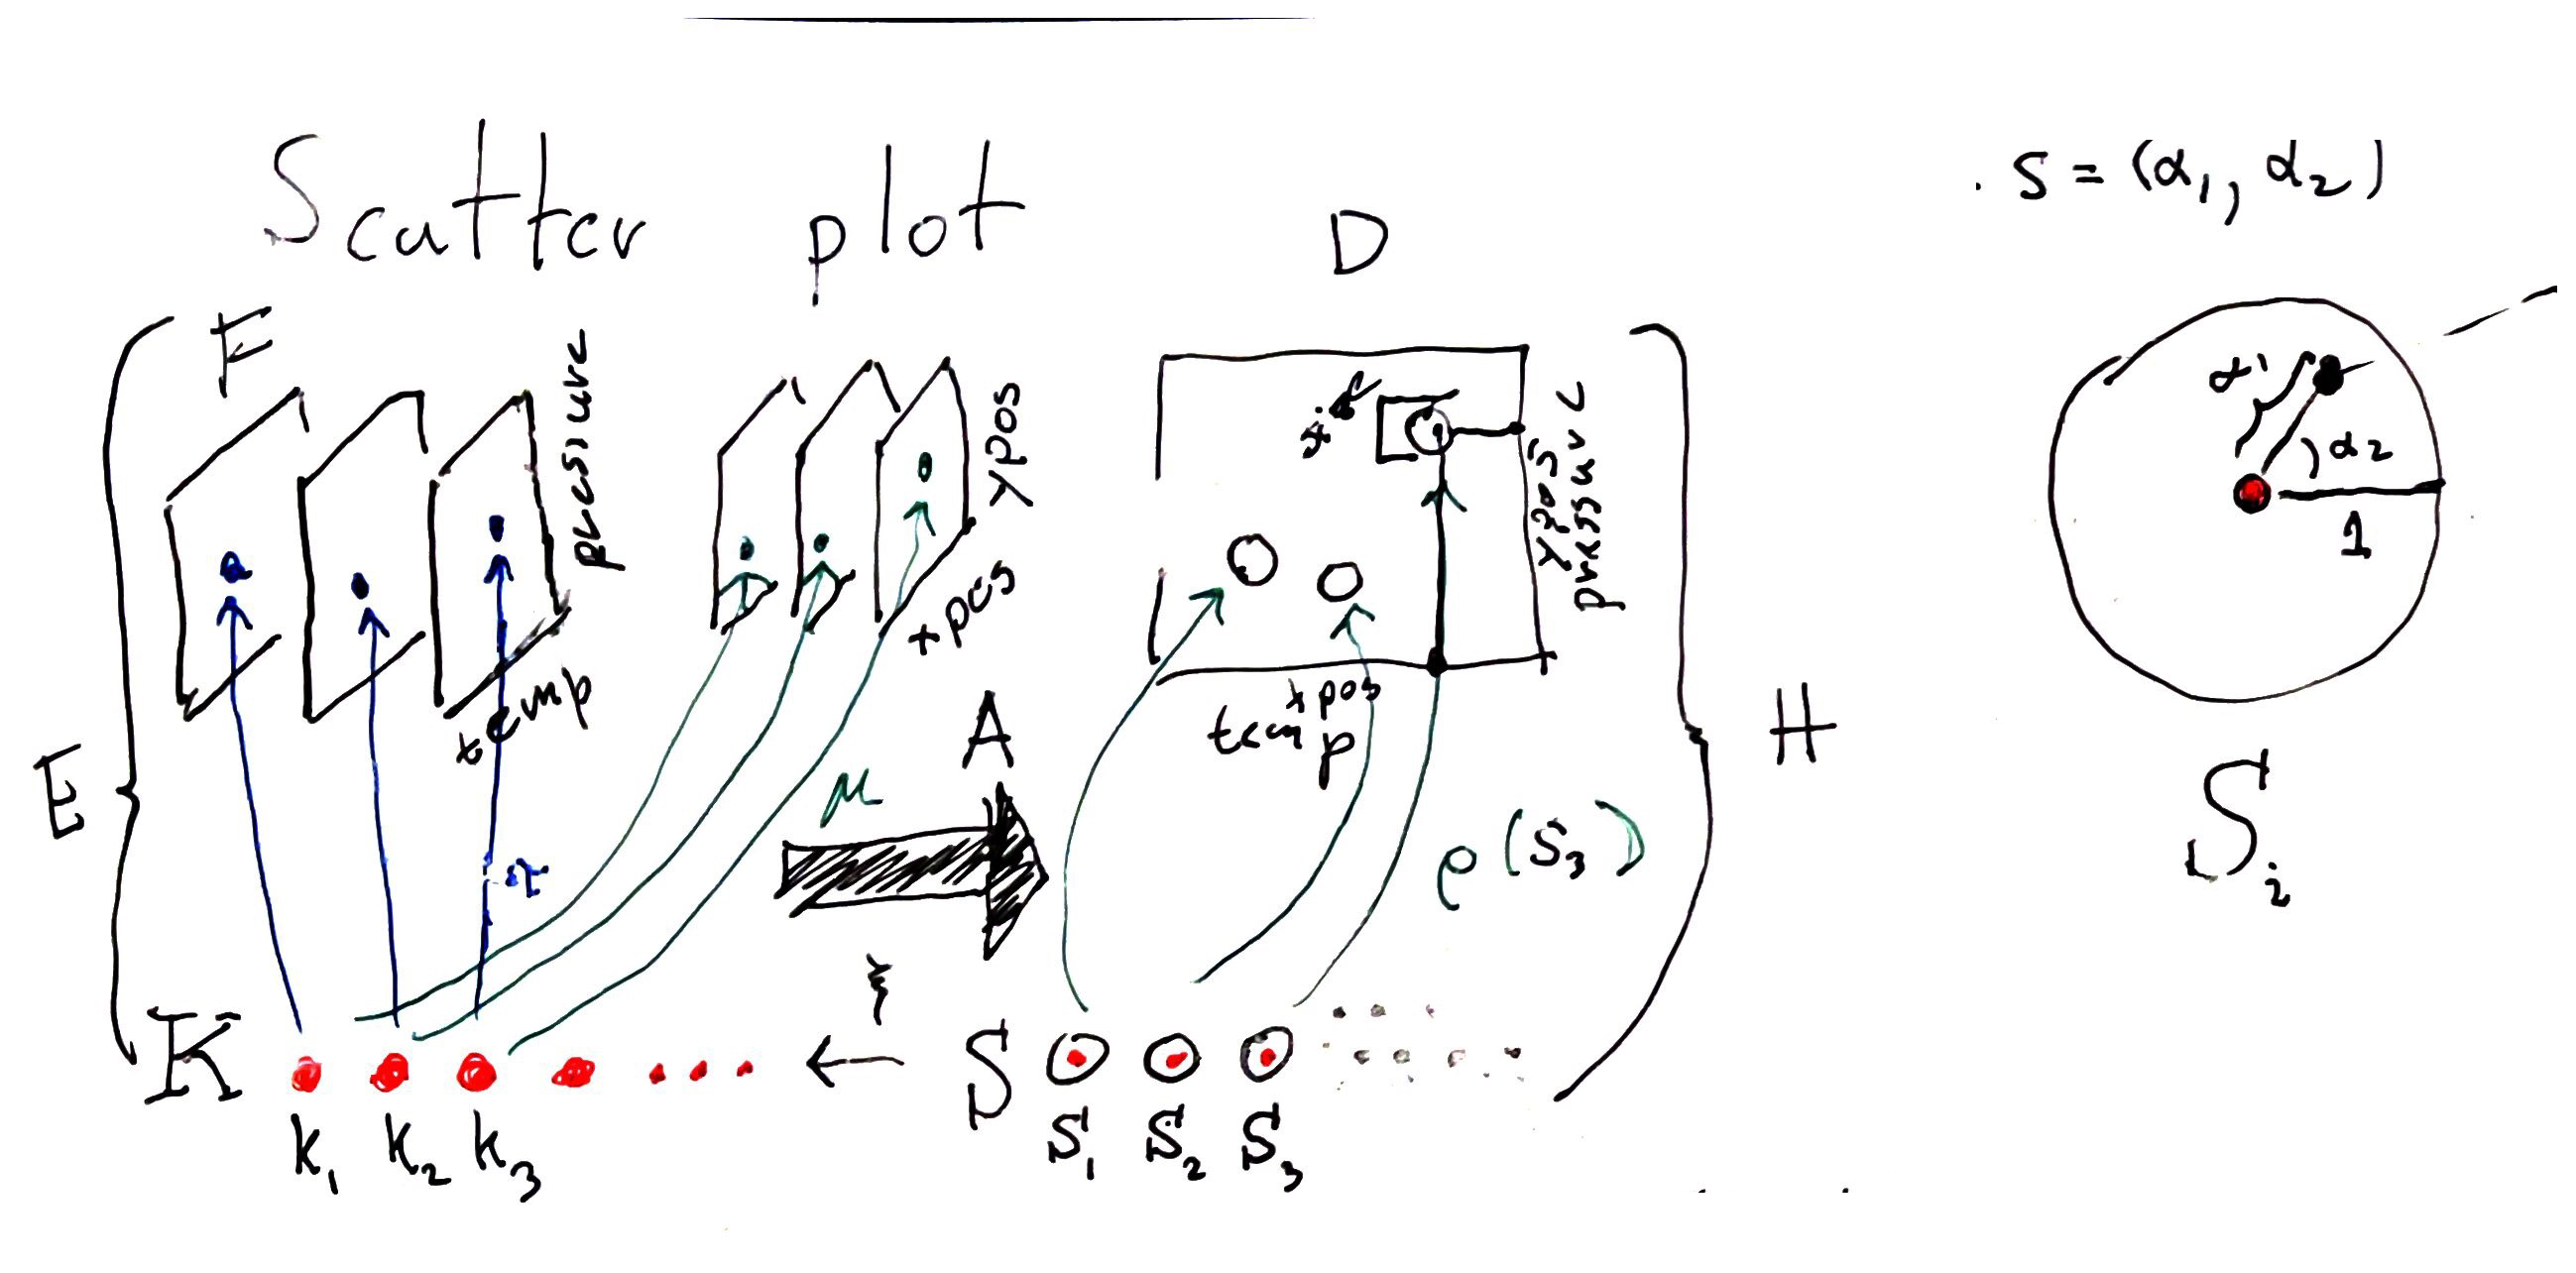
\includegraphics[width=\textwidth]{figures/math/scatter.png}
    \label{fig:artist_scatter}
\end{figure}

\begin{equation}
Q(xpos, ypos)(\alpha_{1}, \alpha_{2}) 
\end{equation}

Given a defaut color of black, $\rho_{RGB} = (0,0,0)$. The position of this swatch of color can be computed relative to the location on the disc $S_{i}$ as shown in figure~\ref{fig:artist_scatter}:
\begin{align}
x &= size\bullet \alpha_1 \bullet \cos(\alpha_2) + xpos\\
y &= size\bullet \alpha_1 \bullet \sin(\alpha_2) + ypos
\end{align}

such that $\rho(s) = (x, y, 0, 0, 0)$ where $s$ is the region in $H$. 

\paragraph{Q: line plot}
\begin{figure}[h!]
    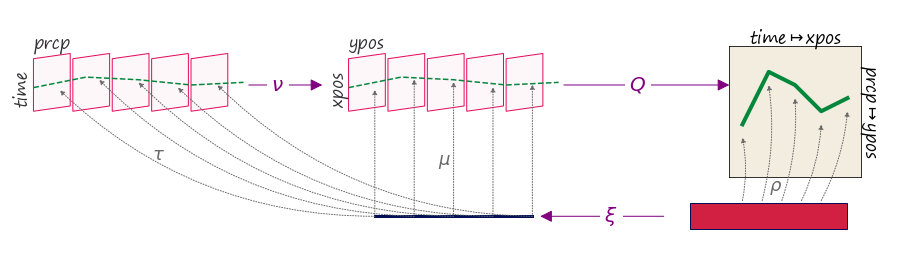
\includegraphics[width=\textwidth]{figures/math/line.png}
    \label{fig:artist_line}
\end{figure}

The line plot shown in fig~\ref{fig:artist_scatter} exemplifies the need for the jet discussed in section~\ref{sec:sheaf_stalk}


\begin{equation}
    Q(xpos, \hat{n_{1}}, ypos, \hat{n_{2}})(\alpha_1, \alpha_2)
\end{equation}

where the magnitude of the thickness is 
\begin{equation}
    \lvert n \rvert = \sqrt{{n_{1}}^2 + {n_{2}}^2}
\end{equation}
such that the components are 
\begin{equation}
    \hat{n_{1}} = \frac{n_1}{\lvert n \rvert}, \; \hat{n_{2}} = \frac{n_2}{\lvert n \rvert}
\end{equation}
    
which yields components of $\rho(s)$:
\begin{align}
 x = xpos(\xi(\alpha_1)) &+ \alpha_2\hat(n_1)(\xi(\alpha_1)) \\
 y = ypos(\xi(\alpha_1)) &+ \alpha_2\hat(n_2)(\xi(\alpha_2)) 
\end{align}


\paragraph{Q: heatmap}
\begin{figure}[h!]
    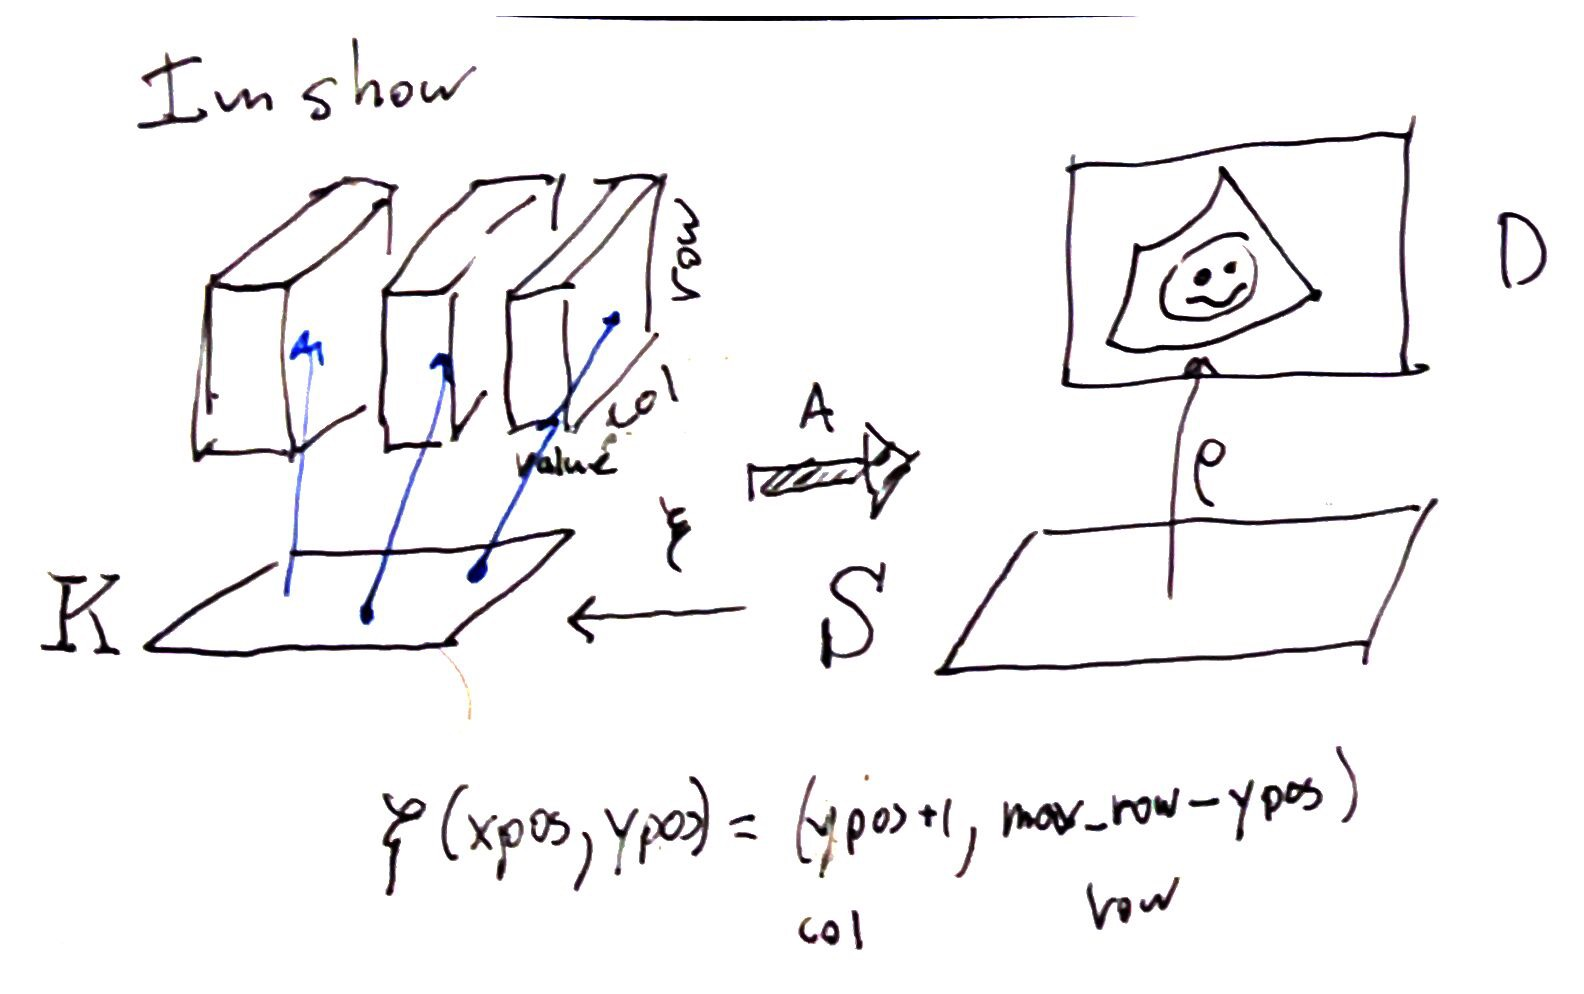
\includegraphics[width=\textwidth]{figures/math/heatmap.png}
    \label{fig:artist_heatmap}
\end{figure}
The heatmap in figure~\ref{fig:artist_heatmap} 
\begin{equation}
Q(xpos, ypos, color)
\end{equation}
has in the simple case a direct lookup into $K$ to obtain the $\mu = (x,y,c)$ values that are mapped into 
\begin{align}
D_{RGB} &= color(\xi(\alpha_1, \alpha_2))
D_x & = xpos(\xi(\alpha_1, \alpha_2))
D_y &= ypos(\xi(\alpha_1, \alpha_2))
\end{align}
through $\rho$. 


\subsection{Making the fiber bundle computable}
\label{sec:triangulization}

\begin{figure}[h!]
    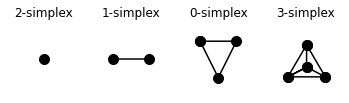
\includegraphics{figures/math/simplex.png}
    \caption{Simplices can encode the connectivity of the data, from fully disconnected (0 simplex) observations to all observations are connected to at least 3 other observations}
    \label{fig:triangle_simplex}
\end{figure}

One way to build flexible $\xi$ is to choose a consistent way of representing$K$. In our draft implementation of the data as fiber bundle model, we triangularize $K$ using complexes of the simplicies shown in figure~\ref{fig:triangle_simplex} such that $\xi$ consistently yields some combination of vertexes, edges, and faces. This gives a common data indexing structure on which to build components that could potentially be reused across $Q$.

\subparagraph{Example}
\begin{figure}[h!]
    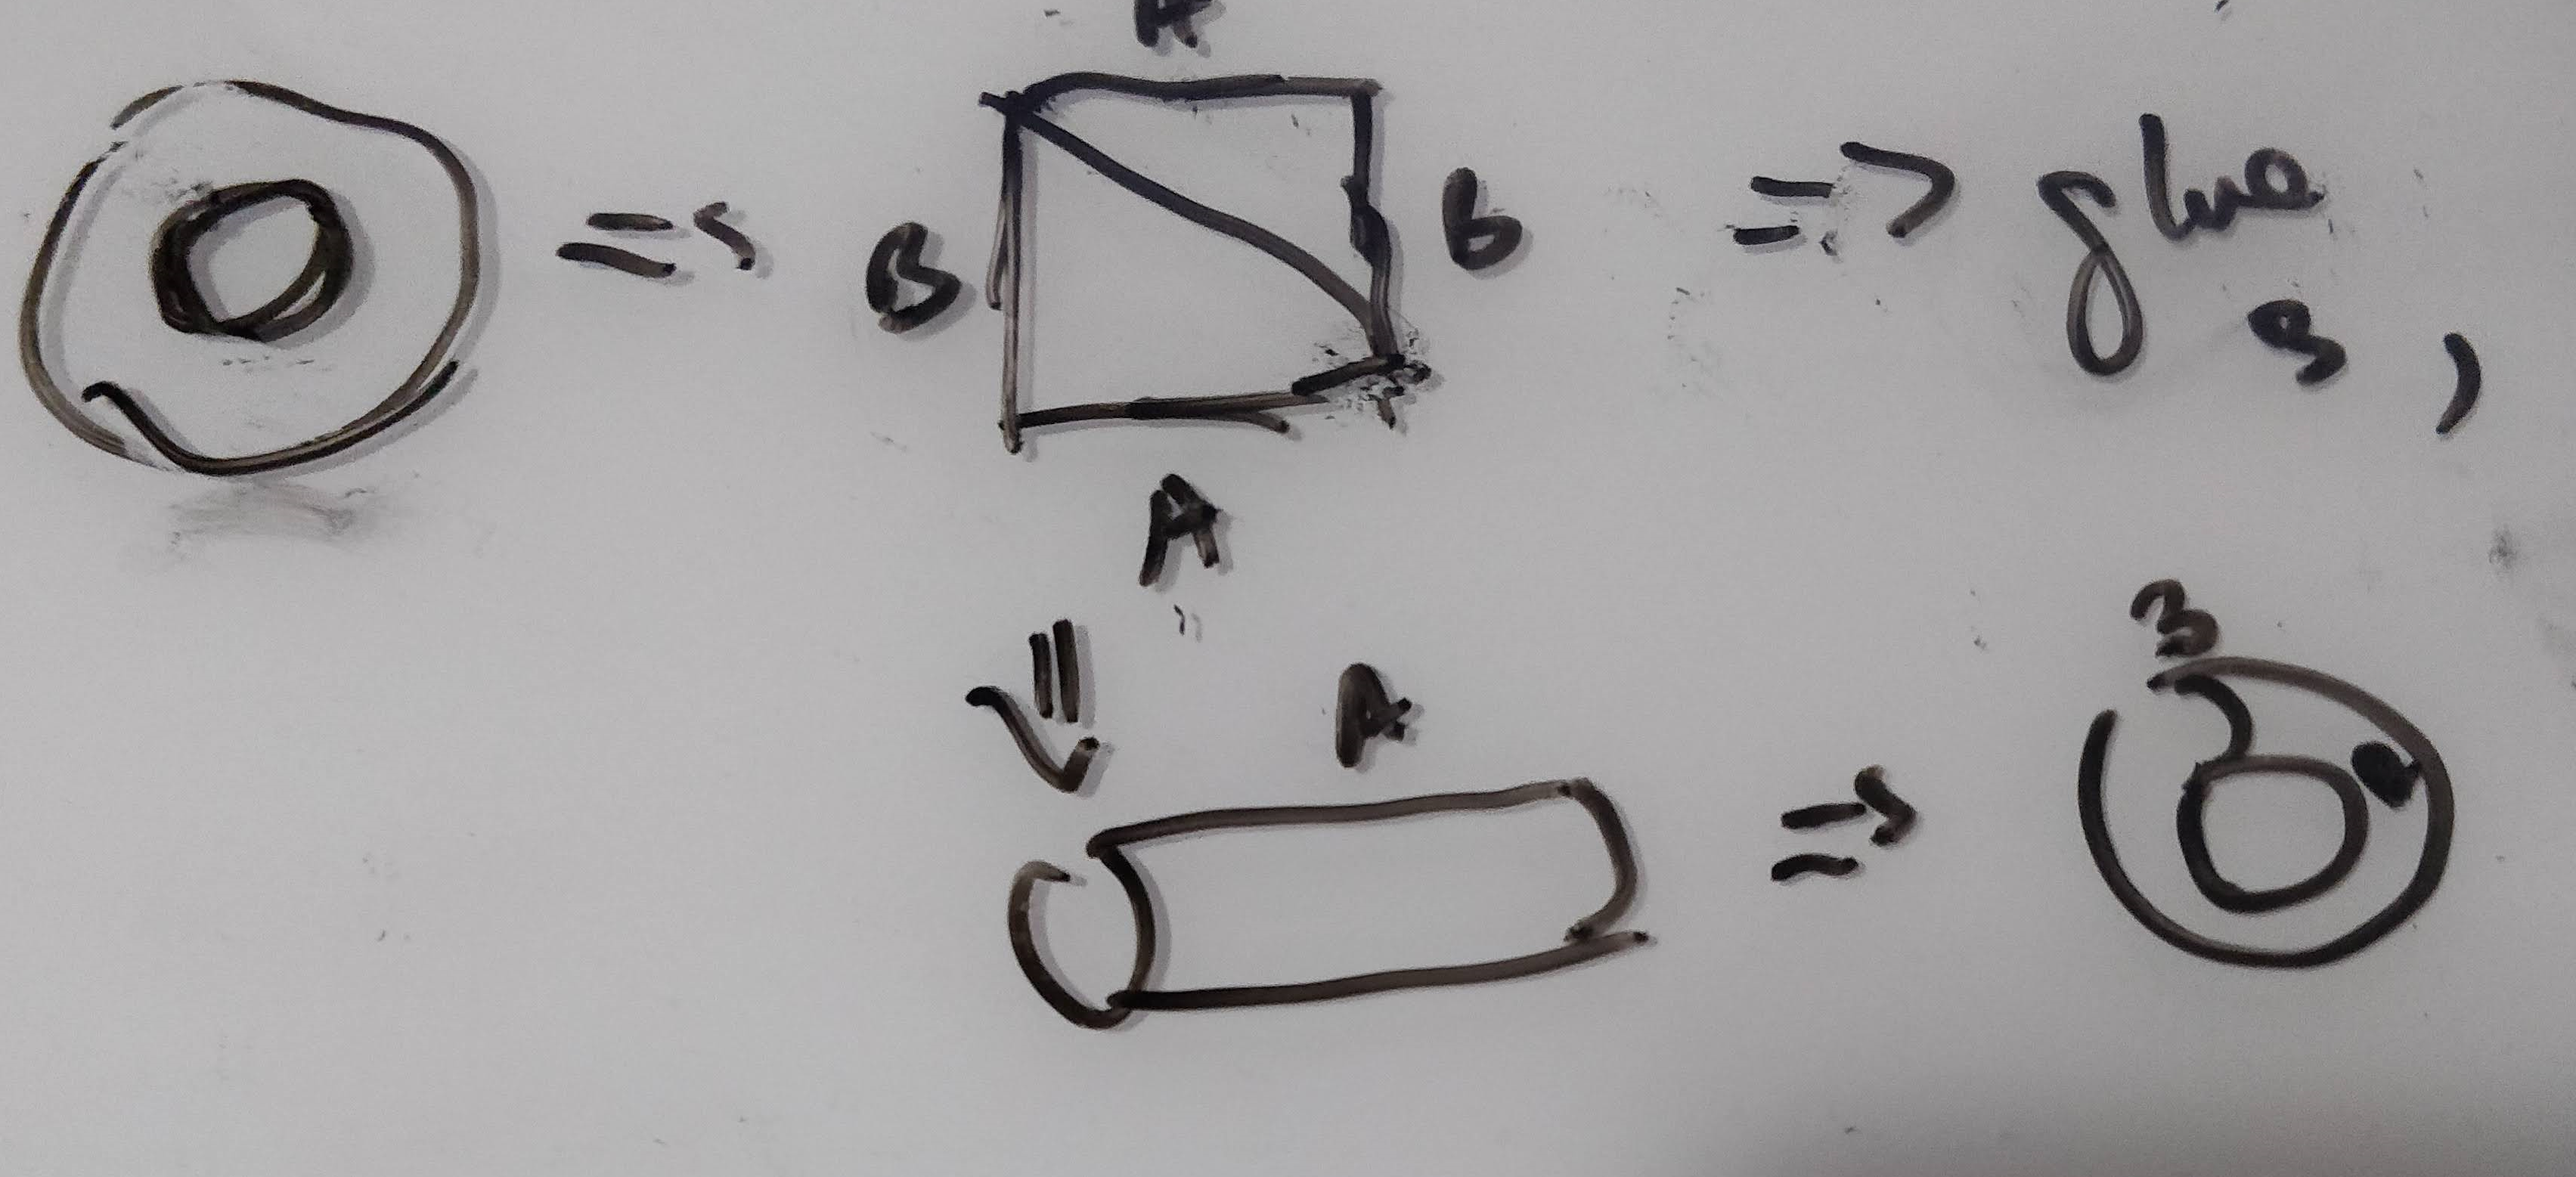
\includegraphics[width=\textwidth]{figures/math/triangle_torus.png}
    \label{fig:triangle_torus}
\end{figure}

Given data that lies on the toroidal space shown in figure~\ref{fig:triangle_torus}, the torus $K$ can be implemented as a simplacial complex of two 2-simplexes. We unfold the torus into the two triangles that compose the square in figure~\ref{fig:artist_heatmap} and encode that as K. We also constrain the functions on $A$, $A^\prime$, $B$ and $B^\prime$ such that $A$ can be glued to $A^\prime$ and $B$ to $B^\prime$ to reconstruct the torus. 

\subsubsection{Visual Idioms: Equivalance class of artists}
As formulated above, every artist function $A$ has fixed $\nu$ and generates a distinct graphic $\rho$. It is unfeasible to implement $A$ for every single graphic; instead we implement the equivalence class of artists $\{A \in A^\prime: A_{1} \equiv A_{2}\}$ which is $Q:\Gamma(V) \rightarrow \Gamma(H)$. 

%% Well maybe. I think this is where required components comes in. There is some minimal V where if you didn't have those variables you wouldn't call it a scatter plot .... something like xpos,ypos with K just a descrete set.
%% so V probably can be any V that contains that sub-bundle
%% so if bubble plot is not the same as scatter plot, and something where the colors change based on data is not scatter plot then it is the equivalent class of something with that minimal bundle.
%% But then if you want to include ANYTHING that also maps with X-Y ... then you hit "direct limits" where you limit over all possivle V_big containing V_minimal
%% You still get a map on some A_minimal -> A_big
%% If you know how to visualize with more variables .. you can always fix them.
\end{document}